\documentclass[]{report}   % list options between brackets


% Latex Police and file encoding
\usepackage[utf8]{inputenc}
\usepackage[T1]{fontenc}  % for character encoding 
\usepackage{lmodern}  % Police setting
\usepackage[frenchb]{babel}


%style of tex :
\setlength{\parskip}{1ex plus 0.5ex minus 0.2ex} %space between paragraphs

% Code Formating
% For code snippets style definition

\usepackage{color}
\usepackage{listings}


\lstloadlanguages{[ISO]C++,C}
% set up listing environment with C syntax hightlight
\definecolor{stringcolor}{rgb}{0.20,0.50,0.20}
\definecolor{commentcolor}{rgb}{0.40,0.40,0.40}
\definecolor{keywordcolor}{rgb}{0.50,0.10,0.10}
\definecolor{idcolor}{rgb}{0.10,0.10,0.50}
\definecolor{bg}{rgb}{0.95,0.95,0.95}
% with \lstset one can predefine parameters for listings
\lstset{language=[ISO]C++,basicstyle=\small,keywordstyle=\color{keywordcolor},
        commentstyle={\color{commentcolor}\itshape},
        stringstyle={\color{stringcolor}},
        identifierstyle=\color{idcolor},numbers=left,
       % xleftmargin=2em,framerule=0.8pt,
        stepnumber=1,frame=single,showstringspaces=false,
        firstnumber=1,numberstyle=\ttfamily,backgroundcolor=\color{bg},
        basicstyle=\footnotesize}
        
        
% Definition of \C++ to be eye candy :
\usepackage{relsize}
\usepackage{lipsum}
%c from texinfo.tex
\def\ifmonospace{\ifdim\fontdimen3\font=0pt }
\def\C++{%
\ifmonospace%
    C++%
\else%
    C\kern-.1667em\raise.30ex\hbox{\smaller{++}}%
\fi%
\spacefactor1000 }

%Inliine listings :
\usepackage{paralist}

%figures :
\usepackage{graphicx}
\usepackage{float}
\floatstyle{boxed} %border around figures
\restylefloat{figure}
\usepackage[format=plain,indention=.5cm,parskip=5pt,bf]{caption}
%import section
\usepackage{wrapfig}

%arays
\usepackage{array}

%
\def \gofigure{{}Gofigure\raisebox{-0.2ex}{2}{}}

%TODO macro
\newcommand{\TODO}[1] {\marginpar{\colorbox{red}{\Huge \textbf{TODO}} } \colorbox{red}{\Huge \textbf{TODO}}\colorbox{green}{\normalsize #1  } } 

% Hypertext links
\usepackage[colorlinks=true,breaklinks=false,dvips,ps2pdf]{hyperref}
\urlstyle{sf}




\begin{document}

\title{Projet de Fin d'Étude}   % type title between braces
\author{Antonin Perrot-Audet}         % type author(s) between braces
\date{April 27, 2010}    % type date between braces
\maketitle

\begin{abstract}
  Ce rapport présente le travail effectué pendant mon Projet de Fin d'Étude au seins du Megason Lab, Harvard Medical School. Ce PFE conclut ma formation à l'Institut National des Sciences Appliquées de Lyon, au département Génie Électrique, pour acquérir le grade d'Ingénieur INSA. Il s'agit aussi d'un stage de recherche finalisant le master Génie Électrique et des Procédés, parcours Systèmes et Images à l'INSA de Lyon, l'École Centrale de Lyon, et l'Université Claude Bernard Lyon 1.
  
  Le travail effectué est porté sur le traitement d'images biologiques. Il s'agit de vidéos tri-dimensionnelles de poisson zèbre durant sa phase de développement embryonnaire. Il s'agissait de trouver des méthodes de segmentation de la paroi cellulaire. Le laboratoire inclut une équipe d'informaticiens développant un programme a l'usage des biologistes : Gofigure2\cite{refGofigure2}. A terme, les résultats théoriques devront être intégrés à cette application.
  
  
\tableofcontents  
  
 
\end{abstract}



\chapter{Description du Megason lab et de ses objectifs} 

\section{Le Megason Lab}

\subsection{L'équipe du laboratoire}
Le Megason lab est un laboratoire dont le personnel est surtout composé de chercheurs post-doctorants.
Il y a clairement deux domaines d'expertise : Biologie, et Informatique.
L'équipe de biologie mène des recherches sur le développement du poisson zèbre,
tandis que l'équipe d'informaticiens développe un programme de visualisation,
segmentation, suivi de cellules adapté aux données de microscopie.

{\small \begin{tabular*}{1.2\textwidth}{@{\extracolsep{\fill}} |  p{2.5cm} |  p{2.6cm} | p{3.3cm} | c | r | }
\hline Nom & Poste & Intérêts & Photo & Nationalité \\ 
\hline Sean Megason & Professeur (Docteur) &  &  &  \\ 
\hline Ramil Noche & Séjour Postdoctoral & Formation du système nerveux. &  &  \\ 
\hline Arnaud Gelas & Ingénieur de recherche (senior) & Programmation de Gofigure2 : Management du projet. &  &  \\ 
\hline Kishore Mosaliganti & Séjour Postdoctoral & Algorithmes de traitement de l'image, recalage et segmentation. &  &  \\ 
\hline Fengzhu Xiong & Étudiant en thèse & Création d'un poisson ayant une couleur différente par cellule. &  &  \\ 
\hline Nikolaus Obholzer & Séjour Postdoctoral & Développement de l'oreille et création de marqueurs génétiques fluorescents. &  &  \\ 
\hline Lydie Souhait & Ingénieur de recherche & Programmation de Gofigure2 : interface graphique et base de donnée. &  &  \\ 
\hline Paul Cowgill & Étudiant en thèse & Effet des drogues sur le poisson zèbre. &  &  \\ 
\hline David Tulga & Étudiant en thèse & Développement cellulaire. &  &  \\ 
\hline Ian Swiburne & Séjour Postdoctoral & Développement de l'oreille du poisson zèbre. &  &  \\ 
\hline Andrea Tentner & Séjour Postdoctoral & Différenciation des cellules provenant d'un ancêtre commun. &  &  \\ 
\hline Dante D'India & Technicien & Entretient des animaux. &  &  \\ 
\hline Nicolas Rannou & Ingénieur de recherche & Programmation de Gofigure2 : intégration de VTK et des algorithmes ITK au programme. &  &  \\ 
\hline Amelia Freen & Séjour Postdoctoral &  &  &  \\ 
\hline Antonin Perrrot-Audet & Stagiaire en PFE & Traitement d'image : Segmentation des cellules; Programmation de Gofigure2 &  &  \\ 
\hline Evan Schwab & Associe & Séquences du code génétique du poisson zèbre. &  &  \\ 
\hline  &  &  &  &  \\ 
\hline  &  &  &  &  \\ 
\hline 
\end{tabular*} }
Il est important de noter que le Megason lab bénéficie des infrastructures et services du département Systems Biology de Harvard Medical School.


\subsection{Les objectifs du laboratoire}
L'objectif principal du Megason lab, est de comprendre les premières étapes du développement animal.
L'idée étant d'interpréter le génome comme un programme informatique.
En modifiant ce dernier, et en observant le développement cellulaire,
les biologistes parviennent à identifier les acteurs intervenant dans le développement de l'embryon, et à comprendre leur fonction.
Les expériences sont réalisées sur des poissons zèbres.
De la même manière qu'un informaticien introduit des "breakpoints" dans un programme pour intervenir dans son exécution,
les biologistes créent des poissons mutants et analysent les effets des modifications du génome sur le développement.
L'étape suivante consistera a créer un modèle du développement du poisson zèbre.
En ce moment, les centres d'intérêts de l'équipe de biologiste sont la formation du tube neural, et des oreilles.

Les biologistes recueillent d'énormes quantités de donnée correspondant a des vidéos d'embryons de poissons zèbre.
Afin de pouvoir exploiter ces données, une équipe de développeurs informatiques a été formée.
Cette équipe a pour objectif de développer la prochaine plateforme pour l'analyse d'images de microscopie: Gofigure2.
Il s'agit donc de créer une application extrêmement accessible ("cross-platform"), avec un code de qualité,
pour permettre l'implication de chercheurs en traitement de l'image, ou d'autres informaticiens ("open-source").

\subsection{Le Matériel} 
Le Megason lab dispose de matériel neuf, tant les outils utilises par les biologistes, que les équipements plus perfectionnes sont très récents et pris en charge par le personnel d'Harvard.
Pour mon PFE, je me suis plutôt intéressé aux dispositifs d'acquisition et de traitement d'image : les microscopes et aux ordinateurs, 

\subsubsection{Les dispositifs d'imagerie}
Le Megason lab dipose de nombreux microscopes pour permettre aux biologistes de mener a bien leurs manipulations sur les poissons zèbre.
L'équipe de traitement de l'image s'intéresse plutôt aux images produites par le microscope confocal deux photons avec plateau automatisé. 

Les techniques d'imagerie au Megason Lab sont basés sur des marqueurs fluorescents fixés sur certaines molécules du spécimen. Ces phosphores doivent être excités afin d'émettre de la lumière.

Le principe du microscope confocal est d'illuminer (exciter) seulement le point que l'on observe : la lentille d'illumination est aussi la lentille d'observation, on illumine donc le plan focal de cette lentille. Cela permet de concentrer l'énergie lumineuse sur le plan observé (plan focal). De plus, afin de limiter l'impact des plans non observés, un diaphragme est ajouté à l'objectif d'observation.

Le microscope confocal dont nous disposons est un microscope deux-photons.
Cela s'signifie que l'illumination du point observée est faite par deux rayons lumineux convergents.
Cette technique a plusieurs avantages :
\begin{itemize}
  \item Le phosphore a besoin de l'énergie de deux photons pour émettre de la lumière. En dehors du point focal, il n'y a jamais assez d'énergie apportée : seul le phosphore focalisé peut émettre de la lumière. On accroit ainsi énormément la résolution.
  \item La longueur d'onde d'excitation est approximativement deux fois plus grande que celle d'un microscope confocal traditionnel, et pénètrent donc mieux les tissus : on peut analyser des spécimens épais.
  \item Chacun de ces deux rayon transporte moins d'énergie que si il y avait eu un seul rayon pour illuminer le point observé.
  Ainsi, il y a moins de dommages causés au spécimen observé.
\end{itemize}

%\begin{figure}[h]
%\begin{center}
%\leavevmode
%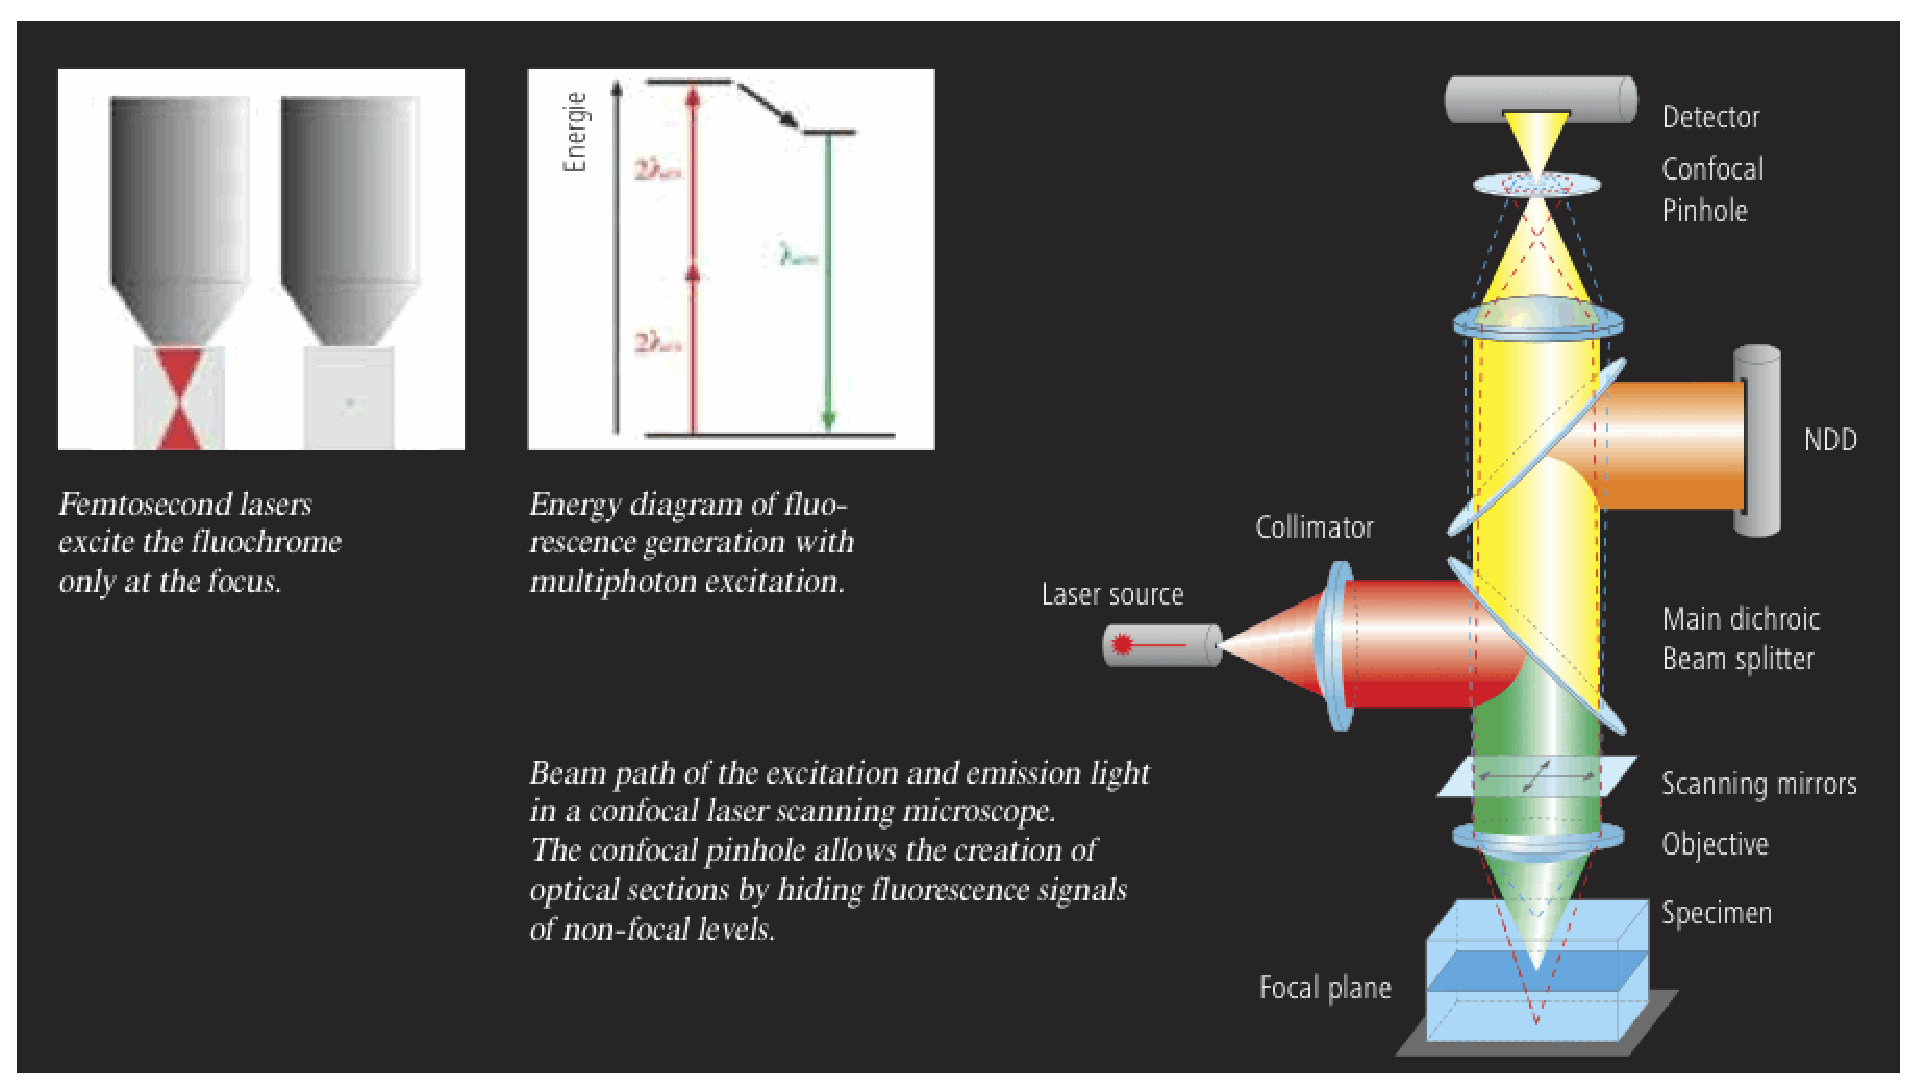
\includegraphics[width=0.95\textwidth]{pictures/ConfocalZeissPrinciple}
%\end{center}
%\caption{Principe du microscope confocal 2 photons utilisé (Zeiss documentation)}
%\label{fig:ConfocalPrinciple}
%\end{figure}
%\TODO[fix image here]
%
% 
% content section
%\begin{wrapfigure}{r}{8cm} % "l" or "r" for the side on the page. And the width parameter for the width of the image space.
%\centering
%\includegraphics[height=80mm]{Abb/bluesniper.jpg}
%\caption{Selbstgebaute „Bluesniper“ um Bluetooth-Geräte aus über 1 km Entfernung anzugreifen. (Stand: 2004)}
%\label{bluesniper}
%\end{wrapfigure}


Il est pour l'instant possible d'utiliser trois canaux différents et donc d'utiliser trois marqueurs fluorescents différents.
Ce microscope a été assemblé au Megason Lab à partir d'un microscope Zeiss 710 NLO.
Une chambre environnementale a été créée, afin de contrôler le développement des embryons durant la capture d'informations.

\TODO[check other microscope]
Nous disposons aussi d'un microscope 

% Chapitre sur le rapport d ingenierie :


\chapter{Rapport d'ingénierie} 


\TODO {ADD definitions to glossary !!!!}






\section{Introduction}

Ce PFE conclut les cinq années d'étude a l'INSA de Lyon. 
Il s'agit de démontrer des capacités d'adaptation, d'innovation et d'initiative propres a un ingénieur. Les laboratoires aux 
États-Unis ont besoin de l'expertise d'ingénieurs pour résoudre des problème techniques. 
Notamment, au Megason Lab, ce sont principalement des ingénieurs qui développent le programme de visualisation de données. 
Les problèmes d'acquisitions d'images biologiques révèlent aussi des défis techniques.
 
\section{Objectifs}

Les objectifs initialement proposés contenaient une très forte composante recherche.
Cependant, le Megason lab cherche au maximum a intégrer les avancées en traitement de l'image aux outils qu'il conçoit,
 notamment au programme Gofigure2. Cela entraine des contraintes vis à vis des outils de développements. 
 Il a donc fallu me former afin que je devienne un programmeur avancé en {\C++}. 
 
J'ai ainsi commencé mon PFE en tant que membre de l'équipe de développement de Gofigure2.
 Les objectifs étant d'apprendre les différentes librairies utilisées par le programme, pour mettre au point un système de plugins. 
 Ma mission était de créer une librairie de comparaison d'images, afin d'inclure aux plugins, un aperçu à la Photoshop.

Dans le cadre de ma participation au développement de Gofigure2,
 j'ai aussi proposé un protocole de travail avec un nouveau programme de contrôle de version : GIT.
 Il s'agissait tout d'abord d'apprendre à utiliser GIT, pour ensuite transmettre ce savoir et enfin proposer une méthode de travail.

Mon PFE étant motivé par des objectifs de traitement de l'image, j'ai aussi travaillé sur l'amélioration
 des techniques d'acquisitions de données microscopiques.





%--------------------------------------------------
%             COMPARAISON
%--------------------------------------------------


\section{Création d'une librairie de comparaison d'images}

L'équipe d'informaticiens au Megason Lab est divisée en deux : deux ingénieurs travaillent sous la direction d'un docteur sur la
 création de l'outil de visualisation d'images microscopiques (GoFigure2), tandis qu'un autre docteur travaille sur
 des algorithmes de traitement d'image. Afin de travailler pour l'ensemble des informaticiens, le projet devait
\begin{inparaenum}[(i)]
  \item faciliter le travail de développement d'algorithmes de traitement de l'image, et 
  \item s'intégrer au développement de GofiGure2.
\end{inparaenum}

La création de la librairie de comparaison d'images atteint ces deux buts : Il s'agit d'un programme utilisant le code source du projet Gofigure2, qui sera utilisé pour le développement des plugins de Gofigure2.
Cette librairie a enfin était spécifiquement développée pour compléter le projet de débugger graphique de Matt McCornicc \TODO{inserer reference Matt}afin de rendre cette librairie particulièrement utile aux traiteurs d'image développant sous ITK. Ce programme permet aussi de visualiser les traitements appliques aux données lors de l'exécution d'un algorithme de traitement d'image sous un environnement de debugging (gdb\TODO{definir GDB}).


\subsection{cahier des charges}

Des objectifs généraux définis en introduction, nous pouvons dégager les fonctions principales de la librairie :
\begin{itemize}
  \item compatible avec ITK
  \item compatible avec VTK
  \item compatible avec Qt
  \item Inclure des classes de Gofigure2
  \item facile a utiliser
  \item bien documentée.
\end{itemize}


\subsection{les outils utilisés}

\subsubsection{Les librairies \C++}
Il existe un grand nombre de fonctions déjà codées en {\C++}. Dans une optique de standardisation et d'efficacité, il est important d'apprendre a utiliser des librairies contenant les fonctions utiles au programme que l'on crée.

Le projet utilise trois grandes librairies :
\begin{description}
  \item[Insight ToolKit (ITK)] qui est spécialisée dans le traitement d'image. Nous utilisons cette librairie, 
  afin de supporter le type de données qu'elle stocke en mémoire.
  \item[Visualization ToolKit (VTK)] qui est spécialisé dans la visualisation d'images. 
  Nous utilisons cette librairie afin de supporter le type de données qu'elle stocke en mémoire,
  et aussi pour visualiser les données acquises par la librairie.
  \item[Qt] qui est spécialisée dans la création d'interface graphiques. 
  Nous avons rendu notre travail directement compatible avec cette librairie
  pour permettre aux utilisateurs de l'intégrer dans n'importe quelle application développée avec Qt.
\end{description}
Une description détaillée de ces librairies est présentée en annexe.

\TODO{Annexe avec description pipelines etc... vtk itk qt}

\subsubsection{Les outils de programmation}
A partir d'un certain niveau, en {\C++}, il est indispensable de maitriser certains outils complexes. Ceux-la, après un temps
 d'apprentissage, augmentent grandement la productivité.
Les outils utilisés quotidiennement, dans le processus de développement d'applications au Megason lab sont :

\begin{description}
  \item[l'Unix Shell] : pratiquement tous les développeurs travaillent sur Linux car ce système inclut un grand nombre d'utilitaires
  standard pour un développement en {\C++}. Les outils de contrôle de version (SVN, GIT), les outils de connexion réseau (ssh), des
  compilateurs pour les principaux langages sont installes par défaut sur la plupart des distributions Linux.
  Afin de pouvoir bénéficier au maximum de ce système, il est important de maitriser l'invite de commande.
  \item[CMake] : ce programme permet de définir des règles de compilation pour différents compilateurs, afin qu'un projet puisse
   compiler sur différents systèmes d'exploitation (Nous programmons des application fonctionnant sur Windows, Linux et MacOs).
  \item[CTest] : Lorsque l'on travaille sur un projet volumineux, il est facile de "casser" le code. L'ajout de certaines fonctionnalités 
  peut modifier le comportement d'autres parties du programme d'une manière imprévue. L'outil CTest est utilisé au Kegason Lab, 
  pour tester la fiabilité du code. Ce programme télécharge régulièrement le code source, le compile, et effectue une batterie de test 
  des fonctionnalités du programme.
  \item[SVN] Gofigure2 les développeurs de Gofigure2 travaillent sur les même fichiers simultanément. 
  Dans ce cadre, il est important de garder une trace des modifications apportées par chacun. Il faut aussi combiner ces changements, 
  et sauvegarder le projet sur un serveur accessible à tous. SVN est un programme de gestion de versions qui rempli toutes ces 
  fonctions.
\end{description}


\subsection{Agenda}

Afin de planifier les tâches accomplies pour mener à bien ce projet, un diagramme de Gantt est présenté.
\TODO{INSERER GANTT pour Comparer }

\subsection{Résultats}

La librairie a été crée et est fonctionnelle. Elle rempli les fonctions présentées en introduction. Un exemple de code est donné en annexe, illustrant l'extrême simplicité d'utilisation de la librairie.
\TODO{insere code snapshot en annexe}
Une interface graphique basique a été crée pour illustrer les fonctionnalités de la librairie :
\TODO{include screenshots}
En plus d'un article dans l'Insight Journal, d'un code abondamment commenté, et d'une panoplie d'exemples, la librairie est délivrée avec une documentation en ligne.
\TODO{inserer exemple documentation}
Afin de prouver la robustesse des classes utilisées, une série de tests automatiques a été crée.
La librairie a été intégrée au code de Gofigure2, au seins de se librairie graphique (QGoGUI), et est en ce moment intégrée au débugger graphique proposé par Matt Mc Cornic.


\subsection{Travail futur}
La librairie de comparaison d'images est un très bonne base à laquelle on peut ajouter de nombreuses fonctionnalités :
\begin{itemize}
  \item Supporter des images vectorielles d'ITK,
  \item intégrer des filtres simples (gradient, inverse, seuillage...),
  \item ajouter un moteur de rendu 3D (par tracé de rayons par exemple...).
\end{itemize}






%--------------------------------------------------
%             GIT
%--------------------------------------------------


\section{Définition d'un protocole de travail sous GIT}

Une partie de mon travail a consisté en la définition de protocoles 
afin d'effectuer certaines tâches d'une manière organisée et répétable. 
J'ai travaillé sur l'élaboration d'un protocole de travail sur GIT pour l'équipe de programmateurs.

Je suis donc passé par une phase de découverte et d'apprentissage pour ensuite écrire un tutoriel 
afin d'expliquer le fonctionnement de GIT a l'équipe informatique. 
J'ai ensuite propose un "workflow" utilisant GIT.

\subsubsection{Le contrôle de version}

Cette partie présente brièvement la gestion de version et les principales solutions existantes.

\paragraph{Le contrôle de version} ou gestion de version consiste en
la création d'un historique des modifications apportées a un projet.
Il est nécessaire de disposer d'un programme à cet effet, surtout lorsque plusieurs personnes travaillent sur le même projet.
Il est ainsi possible de garder trace de toutes les modifications apportées.
Certains programmes de contrôle de version permettent de modifier l'historique en annulant l'effet d'une modification erronée par exemple.

Les programmes récents de contrôle de version sont aussi utilisés pour permettre a plusieurs développeurs de travailler 
sur le même fichier, ou sur des fonctionnalités différentes.
Il existe un vocabulaire particulier au contrôle de version. Pour ce rapport, il est important de comprendre l'analogie de l'arbre couramment utilisée.
Le tronc (trunc) contient généralement la dernière version commune du projet.
De ce tronc, les programmeurs créent des branches pour apporter des changements.
Ces branches sont des copies du tronc.
L'action de sauvegarder dans l'historique les changements apportés au projet est "committer" (to commit).
L'action de fusionner une branche au tronc (et ainsi rapporter tous les changements effectués sur une branche au tronc),
s'appelle le merge.
Dans les  "anciens" programmes de gestion de version, les changements (commits) sont souvent directement faits sur le tronc.
Cela crée des problèmes de conflits (plusieurs utilisateurs auraient changé d'une manière différente le même fichier, par exemple).

Le code source est souvent stocké sur un serveur en ligne. Ainsi, le programme de gestion de version est aussi utilisé
pour publier le code sur internet, par l'intermédiaire de sites spécialisés (Sourceforge, Github, Gitorious, GoogleCode...).

\TODO{Illustration du fonctionnement d'un programme de gestion de version :}



\paragraph{Les deux philosophies de contrôle de version} sont actuellement la gestion de version centralisée et la gestion de version locale.




Il est possible de trouver une comparaison détaillée des deux philosophies à cette adresse :
\TODO{cite adresse \url{http://informatique.in2p3.fr/?q=node/333}}



\paragraph{principales solutions}

\TODO{inserer un tableau avec les principaux clients}

\paragraph{Avantages de Git sur la concurrence}

GIT n'est pas le seul programme de contrôle de version. Son principal concurrent est Subversion.
Cependant il propose de nombreux avantages dont les principaux sont:
\begin{description}
  \item[rapidité] : GIT utilise un protocole de communication très efficace.
  \item[économie] : GIT utilise un algorithme de compression très performant : le code prend ainsi très peu de place.
  \item[développement en commun] : chacun peut travailler sur une sous partie du programme. La création de "branches" est facile et
  rapide. La mise en commun des changements est bien mieux gérée que sur des programmes concurrents comme SVN.
  \item[développement décentralisé] : chacun possède une copie du code et peut travailler sans connexion internet. 
  Si le serveur subit une panne ou est indisponible, tout le monde peut continuer à travailler, et la recréation d'un serveur est triviale.
  \item[Souplesse] : GIT permet de travailler sur un projet utilisant svn en bénéficiant des avantages de la gestion de projet
  décentralisée.
\end{description}


\subsection{Écriture du tutoriel}

Le tutoriel a été écris sur le wiki de Gofigure2. Il s'agit de l'emplacement de prédilection pour les informations 
concernant la programmation et l'utilisation de Gofigure2. Le système du wiki, en plus de proposer une syntaxe simple 
pour créer des pages web formatées, permet aux lecteurs autorisés de modifier le contenu. 
Il existe aussi un système de feedback permettant aux lecteurs ayant mal compris le contenu, de contacter l'auteur.

L'écriture d'un tel tutoriel se fait souvent dans un registre proche du langage familier,
le but étant de simuler des instruction données par un collègue ou un ami. 
Les instruction se doivent d'être relativement brèves, bien souvent le lecteur veut juste appliquer certaines fonctionnalités 
proposées par GIT sans toujours vraiment chercher a comprendre ce qu'il fait. 
Il existe d'autres sources d'informations pour apprendre complètement le fonctionnement de l'application.
Le tutoriel ne se veut donc pas exhaustif, il propose juste une manière qui fonctionne d'utiliser GIT,
a la manière d'un travail dirigé. Il a été écrit pendant ma phase d'apprentissage de GIT. 
Il détaille les principales difficultés et écueils rencontrés. 

Le tutoriel est présent a cette adresse : \\
\url{http://sourceforge.net/apps/trac/gofigure2/wiki/GIT}

\subsection{Proposition d'un protocole de travail}
Il a enfin fallu proposer un workflow (protocole de travail), qui définit la manière dont les programmeurs
doivent apporter des modifications au code source. Il s'agit de proposer un protocole qui :
\begin{enumerate}
  \item n'augmente pas trop la charge de travail,
  \item permette de bien suivre les modifications apportes par chacun. 
  \item permette au responsable du projet de corriger ou supprimer les changements apportes par les développeurs.
  \item corresponde a un standard.
\end{enumerate}
Le workflow proposé a été détaillé par \href{http://nvie.com/about }{Vincent Driessen} sur son \href{http://nvie.com/git-model}{blog}. Ce protocole découle assez naturellement de l'apprentissage de GIT, il est donc simple.

Ce workflow, en plus d'être précisément détaillé, est techniquement viable.

\subsubsection{description du protocole}

Il existe deux branches principales : 
\begin{description}
  \item[\emph{master}] : cette branche store les versions stables du programme.
  \item[\emph{develop}] : cette branche contient la dernière version commune du programme, elle correspond au tronc.
\end{description}
Ces branches sont présentes sur le serveur central. Le développement du programme se fait sur la branche develop, et lorsqu'une version stable est sur le point d'être produite, on sauvegarde l'état d'avancement du projet dans la branche master.

Il existe ensuite une série de branches de support. Ces branches ont une durée de vie limitée, et doivent fusionner avec d'autres branches pour finalement rejoindre develop (le tronc), puis master. Elles ne sont pas forcement présente sur le serveur central, cela dépend des équipes travaillant sur les différentes parties du programme.
\begin{description}
  \item[\emph{feature}] : cette branche contient le développement d'une fonction du programme. Elle est crée à partir de develop, et une fois mature, refusionne avec \emph{develop}.
  \item[\emph{release}] : cette branche permet aux développeurs de travailler sur la correction de bugs, l'interface graphique, l'ajout de tests... les touches de dernière minute, avant la publication d'une nouvelle version du programme. Elle est crée lorsque la branche \emph{develop} contient toutes les fonctions attendues pour la nouvelle version du programme. Elle est créée à partir de la branche develop et une foi mature, fusionne avec la branche \emph{master}, et \emph{develop}.
  \item[\emph{hotfixes}] : cette branche particulière est créée à partir de la branche \emph{master}, lorsque une version publiée du programme contient un bug important qui ne peut attendre la prochaine version pour être corrigé. Elle refusionne avec la branche \emph{master} pour créer des "sous versions" (0.1.1 par exemple, est une sous version de 0.1.0). Cette branche particulière merge aussi avec la branche \emph{develop} pour appliquer la correction aux futures publications, et enfin, la branche \emph{release} si elle existe au moment de la réparation du bug.
\end{description}

Un cycle de developpement normal devient donc, pour un programmeur :
\TODO{creer une figure}
creation d'une branche feature a partir de develop\\
travail sur la branche feature,\\
fusion de feature avec develop\\
xX\\
creation de release\\
travail sur release\\
merge avec master -> RELEASE\\
merge avec develop\\
destruction de release\\
xOn reboucle\\
\\
Oh no ! un bug :\\
creation de hotfix\\
correction du bug\\
merge sur master -> SOUS RELEASE\\
merge sur develop\\
merge sur release (si release existe)\\
destruction de la branche hotfixes\\


Voici une illustration de ce protocole :

\TODO{insert workflow pdf here}

\section{Amélioration des techniques d'imagerie}


acquisitions :
belles
artifacts, bruits
deplacements violents

remedier a ce probleme


Il est aussi important de noter qu'acquérir une image de qualité facilite grandement le travail de reconnaissance de formes et d'objets, en réduisant les près-traitements.

\subsection{Stabilisation de l'acquisition}

\subsubsection{Principe}


\subsubsection{Code}

demarche : evaluation de la metrique
optimisation tps calcul
developpement en visualbasic (windows emule)

\subsubsection{Tests et travaux futurs}
test sur objet inanime
test sur poisson en developpement
developpements futurs :
metrique non rigide ?
tps de calcul ?
wavelets pour downsample ?


\subsubsection{Planning et avancement}













\section{Projet professionnel}

Ce PFE s'inscrit dans un projet professionnel construit durant ma scolarité a l'INSA de Lyon.
Mon inscription a l'INSa de Lyon a été grandement motivée par l'ouverture de l'école a l'international. J'ai ainsi effectue mon stage ouvrier en Afrique du Sud. Profitant d'une première expérience professionnelle a l'international.

Lors de ma seconde année a l'INSA de Lyon, j'ai choisi l'option SCiences et ANglais (SCAN). Cette filière regroupe les élèves ayant un niveau suffisant pour pouvoir suivre la formation généraliste en anglais. Elle s'accompagne d'une bourse pour un bref séjour linguistique dans une université étrangère. J'ai profite de ce financement pour aller au Trinity College en Irelande ou j'ai pu avoir ma première expérience académique a l'étranger.

J'ai ensuite choisi le département Génie Électrique qui permet de bénéficier d'un grand panel de compétences, notamment dans des domaines rattaches a l'électronique et l'informatique.

Continuant l'expérience internationale, j'ai effectué mon stage industriel au Fraunhofer Institute, Center for Manufacturing Innovation, aux États Unis. Ce stage m'a énormément apporte en plus de l'expérience technique. Il s'agissait d'une première immersion dans la culture américaine. C'est après ce stage que j'ai passe le test TOEIC validant un très bon niveau d'expression et de compréhension en anglais, avec un score de neuf cent quatre-vingt sur neuf cent quatre-vingt dix.

Le PFE au Megason lab possède des attraits indéniables : il s'agit d'un stage de recherche perfectionnant mes connaissances en traitement de l'image. Il s'agit aussi d'une expérience internationale dans une université renommée : Harvard Medical School. Ainsi, en plus de prendre plaisir a travailler en recherche, j'ouvre la porte a de nombreuses opportunités professionnelles.

Comme je suis intéressé par les domaines techniques, je compte profiter de l'opportunité de poursuivre mes études pour obtenir un doctorat en mathématiques appliquées, au cours d'une thèse élaborée en collaboration avec le laboratoire CREATIS (INSA Lyon) et le laboratoire Megason (Harvard Medical School). Cette incroyable opportunité professionnelle est financée en partie par Harvard Medical School et en partie par l'INSA de Lyon. Je passerai ainsi la moitié de mon temps en France, et l'autre moitie aux États Unis.
En plus de pouvoir travailler sur un domaine passionnant, je pourrai ainsi bénéficier d'une équivalence avec un PhD () (diplôme très reconnu a l'international). 

Je compte ensuite mettre en valeur ma capacité a travailler dans un contexte international, dans des domaine a haute technicité pour travailler dans le secteur privé. Je pourrai mettre en avant mes capacités en traitement du signal pour travailler dans le médical ou l'aéronautique.

Mon ambition est de migrer vers des responsabilités manageriales après avoir une très bonne maitrise de la technique.








\section{ANNEXES}



\paragraph{La librairie "Insight ToolKit" (ITK)} est un projet open source initialement destiné au recalage et a la segmentation d'images medicales. ITK a été programmée en \C++ , en utilisant des techniques de codage avancées (templates, modification de la syntaxe standard et ajout de fonctionnalités au langage \C++ par le biais d'idiomes) , ainsi que l'outil de développement cross-platform CMake, et communautaires (SVN, puis GIT). 
Cette librairies est construite sur un système de "Templates", qui lui permet de s'adapter à diverses données. Elle propose une architecture centrées sur un flux de données, traité par différents filtres que l'on connecte ensemble.
Cette collection d'algorithmes ne cesse de s'agrandir grâce à la philosophie open-source. Le spectre des applications d'ITK inclut entre autres exemples:  
\begin{itemize}
  \item l'imagerie medicale, avec \href{http://www.slicer.org/}{3DSlicer},
  \item l'imagerie biologique, avec \href{http://gofigure2.sourceforge.net/}{Gofigure2},
  \item et l'imagerie satellite, avec l'\href{http://www.orfeo-toolbox.org/otb/}{Orfeo ToolBox}.
\end{itemize}
Le modèle de programmation est relativement complexe et nécessite de un long apprentissage, et de l'expérience. A cette fin, de nombreux outils d'information sont mis a la disponibilité du nouvel utilisateur :
\begin{itemize}
  \item des listes de diffusions d'Emails, pour mettre en contact les nouveaux utilisateurs d'ITK et les programmeurs et utilisateurs avancés;
  \item un wiki (\url{http://www.vtk.org/Wiki/ITK}), qui donne quelques informations quand à la mise en place d'un environnement de développement utilisant ITK.;
  \item un guide d'utilisateur très bien expliqué, mais basé sur la version 2.4 d'ITK tandis que la dernière version publiée est la 3.20;
    \TODO {reference ITK software guide}
  \item la documentation Doxygen présentée sous forme de site internet, est directement compilée a partir du code source. Elle est donc plus ou moins complète selon les fichiers. Afin de pouvoir naviguer dans cette dernière, il est indispensable de connaitre la structure du projet.
\end{itemize}
Luis Ibáñez, a dit cette année : "La courbe d'apprentissage d'ITK en \C++ est bien trop raide, et nous allons nous efforcer dans les futures version, de rendre la librairie plus accessible.". La prochaine version d'ITK (version 4) sera donc surement plus facile a utiliser et prendre en main.

\paragraph{La librairie VTK} est développée par Kitware, Il s'agit d'une librairie \C++ utilisee pour la visualisation de données. Elle est open source et cross-platform. Elle utilise des outils similaires a ceux utilises pour ITK (CMake)
Elle utilise un systeme de "pipeline" (flux de donnees) similaire a celui d'ITK pour traiter les donnees a visualiser. Elle est developpee conjointement avec ITK, et il est possible plus ou moins facilement de connecter les filtres de traitement d'image d'ITK avec les filtres de visualisation de VTK.

\paragraph{La librairie Qt} permet une gestion avancée de l'interface utilisateur, en proposant une interface graphique open source et cross-platform.
Elle étend aussi les fonctionnalités du langage \C++ en proposant une nouvelle architecture pour le système de callbacks, un nouveau modèle d'objet, et d'héritage. Cependant, ces modifications sont facilement intégrées par le développeur débutant, grâce a une aide abondante composée d'un ensemble de tutoriels, d'exemples fortement documentes, et d'une liste de diffusion très active.







\section{definitions}




Templates : En programmation informatique, les templates sont une particularité de la programmation en language C++, qui autorise l'écriture d'un code sans considération envers le type des données avec lesquelles il sera finalement utilisé. Les templates supportent la programmation générique en {\C++}.

Cross-platform : Un logiciel multiplate-forme ou multiplateforme est un logiciel conçu pour fonctionner sur plusieurs plates-formes, c’est-à-dire le couple liant ordinateur et système d’exploitation. En anglais on parle souvent de "cross-platform software" ou "platform independent software" ou encore de "multi-platform software".

Idiomes (programmation) :  Un idiome en programmation qualifie un code qui ajoute des fonctionnalités non existantes dans un
langage.

Wiki : Un wiki est un site web dont les pages sont modifiables par tout ou partie des visiteurs du site. Il permet ainsi l'écriture et l'illustration collaboratives de documents.

Graphical User Interface (GUI) : Un environnement graphique est, en informatique, ce qui est affiché en pixels sur un moniteur
d'ordinateur et sur lequel l'utilisateur peut agir avec différents périphériques d'entrée comme le clavier ou la souris. 
Des images, des animations (en 2 ou 3 dimensions), et même des vidéos peuvent être rendues à l'écran.
Ce type d'interface Homme-machine s'oppose à la notion de ligne de commande.

Callback : la technique des fonctions de rappel (callback functions) permet de passer en argument d'une fonction, une autre fonction. 
Cette technique est utilisée dans la programmation évènementielle, ou les interactions de l'utilisateur doivent entrainer l'exécution de fonctions.

\subsection{biblio}

Evaluation/comparaisons de GIT :
descritpion comparaison centralisee non centralisee
\url{http://informatique.in2p3.fr/?q=node/333}
avantages de GIT :
\url{http://www.whygitisbetterthanx.com/}
\url{http://joshcarter.com/productivity/svn_hg_git_for_home_directory}
\url{http://dev-heaven.net/wiki/20/Git_vs_SVN_comparison}

Matt Mc Cornick




% Chapitre sur le rapport de recherche :


\chapter{Rapport de recherche} 

\section*{Introduction}

\subsection*{}
Je présente dans cette partie, la démarche recherche que j'ai eue pendant le PFE. Il s'agit tout d'abord de bien prendre connaissance du sujet. Cette prise de connaissance permet de voir quels problèmes restent à résoudre. Il faut ensuite trouver une solution à ces problèmes, afin de pouvoir avancer dans leur résolution.

La difficulté en recherche, est que bien souvent, il n'existe pas encore de solution dans le domaine étudié.
Il faut donc passer par une phase de bibliographie, pour étudier l'état de l'art,
et éventuellement apprendre de nouvelles théories.
Le domaine du traitement de l'image est une science particulière car beaucoup d'algorithmes sont inventés,
mais très peu sont diffusés ou applicable a divers types d'images.
Il faut donc reprogrammer les algorithmes présentés dans les publications scientifiques et vérifier leurs performances.
Il faut enfin trouver des idées innovantes pour résoudre les problèmes posés, et expérimenter.

\subsection*{}
J'ai travaillé, pendant mon PFE au Megason Lab sur la segmentation d'images obtenues par microscopie fluorescente.
Les données sont quadri-dimensionnelles (espace et temps), et représentent des régions du poisson zèbre (oreille, colonne vertébrale...). Il s'agit de vidéos prises pendant le développement du spécimen. Nous pouvons bien discerner les différentes cellules du poisson, ainsi que leur noyaux. Ces éléments sont donc la base du modèle que nous tentons de créer. Il faut donc être en mesure de détecter et suivre ces cellules au cours du temps. Le modèle devra aussi intégrer les informations morphologiques de chaque cellule.

Ce modèle fait l'objet d'une proposition de thèse : Modèle numérique cellulaire de poisson zèbre ( cells lineage registration in microscopy) durant laquelle j'aimerais poursuivre mes travaux.

Avant d'arriver au Laboratoire, j'ai travaillé sur la membrane cellulaire. J'ai ensuite concentré mes recherches sur la détection et la localisation de noyaux.

\section{Segmentation de la membrane cellulaire par ensembles de niveaux}

Le but initial du PFE etait la segmentation de la membrane cellulaire. il s'agit d'une fine membrane séparant les multiples cellules. Elle s'étend sur tout le spécimen à analyser. Il s'agit donc d'un volume important et complexe.

\subsection{Étude du problème}

J'ai tout d'abord cherché à comprendre le problème posé : sur quelles données allaient se baser la détection, existe-t'il des solutions pour segmenter ce genre de données.

\subsubsection{Les données}
Les images sont acquises a travers un système optique. L'excitation par un laser entraine la fluorescence de certaines parties de la cellule, marquées par une molécule émettant de la lumière dans un spectre dépendant du marqueur utilisé.

Le système a donc une réponse impulsionelle bien visible dans les données. Un point correspond grossièrement a une gaussienne étalée dans les trois dimensions de l'espace, et plus particulièrement selon l'axe perpendiculaire au plan de focalisation.

Il existe aussi un bruit dû au dispositif électronique d'acquisition. De plus, la fluorescence n'étant pas répartie de manière homogène, il existe des "trous" et de la saturation dans les données.
\TODO{inserer des images illustrant les problemes}


J'ai choisi de me focaliser sur trois difficultés afin de trouver des solutions :
\begin{description}
  \item [problème du bruit] : quel filtrage appliquer aux images, afin de les débruiter.
  \item [problème de l'absence de données] : comment introduire des à priori de forme de la membrane
  pour palier à l'absence d'information ?
  \item [problème de la non homogénéité des intensités]  : comment segmenter un objet
  qui n'occupe pas les mêmes intensités selon sa position dans l'espace.
\end{description}


\subsection{Débruitage des données}
Le bruit présent sur les images n'est pas gaussien. Il n'est pas répartis de la même manière dans toute l'image non plus. Je me suis donc focalisé sur des techniques de débruitage telles que le filtre médian, et plus généralement des filtres morphologiques.

Le filtre médian donne de bons résultats

\subsection{Segmentation de la membrane}

\subsubsection{Utilisation de la théorie des ensembles de niveaux}

L'outil choisi pour segmenter la paroi cellulaire, est base sur les ensembles de niveaux (levels-sets). Cette théorie consiste en l'évolution d'un front. Cette évolution est représentée par une fonction implicite qui évolue itérativement. Le front (bords de la zone segmentée) est souvent représenté par le niveau zéro de cette fonction implicite.
Les Level sets, au travers de leur critère d'évolution, permettent d'avoir une grande flexibilité quand aux mesures a considerer lors de l'evolution du front. Cette évolution est représentée par un critère d'énergie, le problème de segmentation par level set est donc un problème d'optimisation.

\subsection{des idees}






idee de la mediane
idee morphologie
idee localisation
\subsection{resultats}
idee mediane
idee morphologie
idee localisation
\subsection{travail futur}
rapidite



\section{Detection et localisation des cellules}

Nous basons nos méthodes de segmentation sur une initialisation au centre des cellules. Nous avons donc besoin de détecter un maximum de cellules afin de trouver un point a l'intérieur de ces dernières. Des methodes ont ete proposees, cependant, chacune est adaptee a un type d'image particulier.
Cels algorithmes de détection sont aussi souvent appelles algorithmes de "seeding" car ils permettent d'obtenir des points a partir desquels une segmentation peut etre initialisee, afin de delimiter les bordures des noyaux, ou les membranes cellulaires.

\subsection{demarche}

Nous avons developpe une methode combinant l'information provenant des noyaux et de la membrane des cellules. Cette methode doit etre evaluee, donc comparee a d'autres methodes existantes. Ce processus d'evaluation nous permettra aussi de trouver les points forts et les points faibles des algorithmes. Nous pourrons ainsi eventuellement utiliser des techniques de fusion d'information pour combiner les resultats de differents algorithmes.
La creation d'un "framework" d'evaluation passe donc par plusieurs etapes : l'implementation des algorithmes existants, afin de les tester sur des images synthetiques puis reelles, la creation de criteres d'evaluation appropories, et l'observation des resultats. Nous avons aussi initié un travail afin de proposer une nouvelle methode de detection de cellules basee sur la decomposition en ondelettes.


\subsection {description des algorithmes evalues}



\subsubsection{chaine de traitement de l'image}

partie commune
Nous nous focalisons sur une classe d'algorithmes traitant l'information issue de l'image des noyaux cellulaires, apres une detection des zones d'interet (binarisation de l'image). Ces algorithmes fonctionnent aussi souvent avec une extraction de maxima locaux en dernier traitement.
Nous choisissons d'utiliser la même binarisation, et la meme methode d'extraction de maximas locaux pour les deux algorithmes afin de focaliser l'etude sur la technique de detection des centres des noyaux.

\subsubsection{description des algorithmes}
\paragraph{le Laplacien de la Gaussienne ameliore}
Nous avons decide d'implementer l'algorithme presente dans \cite{al2009improved}. La methode utilisee est celle du Laplacien de la Gaussienne (LoG). Une methode eprouveee qui s'est montree tres robuste dans d'autres applications telles la detection de points de reperes pour le recallage photographique.



\paragraph{Kishore}

\TODO{Ask Kishore more infos}


\subsection {evaluation}
%\begin{tabular}{|c|c|c|c|c|}
%\hline  & Matching & UnMatching & Missed & Accuracy \\ 
%\hline A1 & 10 & 3 & 1 & 71% \\ 
%\hline A2 & 9 & 2 & 3 & 64% \\ 
%\hline 
%\end{tabular} 



\subsection {conclusion}


\subsection {proposition}



\subsection {planning}


\subsection{resultats}

\subsection{proposition}






\appendix

%Annexes du rapport d'ingénierie



\chapter{Librairies utilisées pour le projet de Comparaison d'images}
\label{AnnexeDescriptionITKVTKQT}


\section*{La librairie "Insight ToolKit" (ITK)} 
ITK est un projet open source initialement destiné au recalage et à la segmentation d'images medicales.

ITK a été programmée en \C++ , en utilisant des techniques de codage avancées (templates
\footnote{Les templates sont une particularité de la programmation en language C++, qui autorise l'écriture d'un code sans considération envers le type des données avec lesquelles il sera finalement utilisé. Les templates supportent la programmation générique en {\C++}.}
, modification de la syntaxe standard et ajout de fonctionnalités au langage \C++ par le biais d'idiomes
\footnote{Idiomes (programmation) :  Un idiome en programmation qualifie un code qui ajoute des fonctionnalités non existantes dans un langage.}
).
ITK utilise aussi l'outil de compilation cross-platform CMake et des outils de développement communautaires (CVS, puis GIT). 
Cette librairies est construite sur un système de "Templates", qui lui permet de s'adapter à diverses données. Elle propose une architecture centrée sur un flux de données, traité par différents filtres que l'on connecte ensemble.
Cette collection d'algorithmes ne cesse de s'agrandir grâce à la philosophie open-source. Le spectre des applications d'ITK inclut entre autres exemples:  
\begin{itemize}
  \item l'imagerie medicale, avec \href{http://www.slicer.org/}{3DSlicer},
  \item l'imagerie biologique, avec \href{http://gofigure2.sourceforge.net/}{Gofigure2},
  \item l'imagerie satellite, avec l'\href{http://www.orfeo-toolbox.org/otb/}{Orfeo ToolBox}.
\end{itemize}
Le modèle de programmation est relativement complexe et nécessite un long apprentissage, et de l'expérience. A cette fin, de nombreux outils d'information sont mis à la disponibilité du nouvel utilisateur :
\begin{itemize}
  \item des listes de diffusions d'Emails, pour mettre en contact les nouveaux utilisateurs d'ITK et les programmeurs et utilisateurs avancés;
  \item un wiki (\url{http://www.vtk.org/Wiki/ITK}), qui donne quelques informations quand à la mise en place d'un environnement de développement utilisant ITK;
  \item un guide d'utilisateur\cite{ITKSoftwareGuide} très bien expliqué, mais basé sur la version 2.4 d'ITK tandis que la dernière version publiée est la 3.20;
  \item la documentation Doxygen présentée sous forme de site internet, est directement compilée à partir du code source. Elle est donc plus ou moins complète selon les fichiers. Afin de pouvoir naviguer dans cette dernière, il est indispensable de connaitre la structure du projet.
\end{itemize}
Luis Ibáñez, a dit cette année : "La courbe d'apprentissage d'ITK en \C++ est bien trop raide, et nous allons nous efforcer dans les futures versions, de rendre la librairie plus accessible.". La prochaine version d'ITK (version 4) sera donc sûrement plus facile à utiliser et à prendre en main.

\section*{La librairie "Visualization ToolKit" (VTK)} est développée par Kitware, Il s'agit d'une librairie \C++ utilisee pour la visualisation de données. Elle est open source et cross-platform. Elle utilise des outils similaires à ceux utilisés pour ITK (CMake)
Elle utilise un système de "pipeline" (flux de donnees) similaire à celui d'ITK pour traiter les données a visualiser. Elle est développée conjointement avec ITK, et il est possible plus ou moins facilement de connecter les filtres de traitement d'image d'ITK avec les filtres de visualisation de VTK.

\section*{La librairie Qt} permet une gestion avancée de l'interface utilisateur
\footnote{Graphical User Interface (GUI) : Un environnement graphique est, en informatique, ce qui est affiché en pixels sur un moniteur
d'ordinateur et sur lequel l'utilisateur peut agir avec différents périphériques d'entrée comme le clavier ou la souris. 
Des images, des animations (en 2 ou 3 dimensions), et même des vidéos peuvent être rendues à l'écran.
Ce type d'interface Homme-machine s'oppose à la notion de ligne de commande.}
, en proposant une interface graphique open source et cross-platform.
Elle étend aussi les fonctionnalités du langage \C++ en proposant une nouvelle architecture pour le système de callbacks
\footnote{Callback : la technique des fonctions de rappel (callback functions) permet de passer en argument d'une fonction, une autre fonction. 
Cette technique est utilisée dans la programmation évènementielle, ou les interactions de l'utilisateur doivent entrainer l'exécution de fonctions.}
, un nouveau modèle d'objet, et d'héritage. Cependant, ces modifications sont facilement intégrées par le développeur débutant, grâce à une aide abondante composée d'un ensemble de tutoriels, d'exemples fortement documentés, et d'une liste de diffusion très active.

\chapter{Script de synchronisation SVN-Git}
\label{AnnexeScriptGIT}

Pour une mise en page correcte, les commandes longues ont été coupées. La coupure est indiquée par un "\verb+\+".

  \begin{lstlisting}[language=bash,title={Script de synchronisation SVN-Git\\exécuté sur le serveur "rainbowfish" localisé au Megason Lab }, label=GitSVNBash]{Bash Script pour la mise à jour de Git à partir du serveur SVN}
#!/bin/bash

cd /Users/arnaud/GITROOT/GoFigure2

#setup environment :

GITBIN=/opt/local/bin
SVNBIN=$GITBIN
SSHBIN=$GITBIN

#update the repository :

echo "**Fetch from svn"
echo `$GITBIN/git svn fetch`
echo `$GITBIN/git svn rebase`

# compress the repository
echo `$GITBIN/git gc`

# convert tags branches created by git svn to real git tags
echo "****Convert tag branches to actual git tags"
for GITREF in `$GITBIN/git for-each-ref refs/remotes/tags \
    | cut -d / -f 4-`; do
  echo "dealing with tag $GITREF"
  $GITBIN/git tag -a "$GITREF" \
      -m"delete SVN" "refs/remotes/tags/$GITREF"
  $GITBIN/git push origin ":refs/heads/tags/$GITREF"
  $GITBIN/git push origin tag "$GITREF"
done

echo "**Push svn:trunk to git:develop"
# first push the trunk to develop
  echo `$GITBIN/git checkout -b develop trunk`
  echo `$GITBIN/git checkout develop`
  echo `$GITBIN/git svn fetch`
  echo `$GITBIN/git svn rebase`
  echo `$GITBIN/git push origin develop`

#then push the branches

#we list the braches currently present on the svn server :
for SVNBRANCHES in `$SVNBIN/svn list \
    http://gofigure2.svn.sourceforge.net/svnroot/gofigure2/branches\
    | sed 's_\/__'`; do

  #which branch are we dealing with :
  echo "****$SVNBRANCHES : fetching from svn"
  #fetch svn branches
  echo `$GITBIN/git svn fetch`

  # create branches linked to remote tracking branches
  # present on the svn server
  echo "  $SVNBRANCHES : try to create git:feature_$SVNBRANCHES \
      and track git remote tracking branch remotes/$SVNBRANCHES"
    echo `$GITBIN/git checkout -b feature_$SVNBRANCHES $SVNBRANCHES`
    echo `$GITBIN/git checkout feature_$SVNBRANCHES`

  #push the branch to origin (github)
    echo `$GITBIN/git push origin feature_$SVNBRANCHES`
done
\end{lstlisting}


\chapter{Diagramme de Gantt global du PFE}
\label{AnnexeGanttGlobal}

\begin{figure}[h]
\begin{center}
\leavevmode
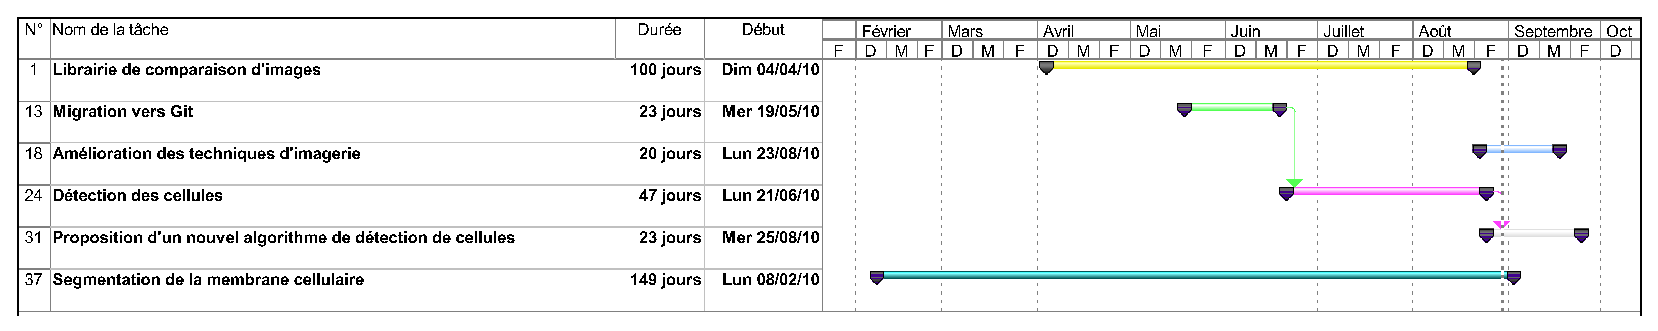
\includegraphics[ width=0.7\textheight, angle=-90,]{pictures/GanttPFE}
\end{center}
\caption{Gantt global du PFE}
\label{fig:GanttPFEGlobal}
\end{figure}


\bibliographystyle{plain}
\bibliography{AntoBib}

\end{document}
